\chapter{Throughput limitation of the Lightning network}

\label{Chapter08HTLClimit}

In this Section, we describe an inherent limitation on the number of concurrent payments Lightning channels can handle.\footnote{This Chapter is based on~\cite{Tikhomirov2020a}.}

Due to the size limitations on Bitcoin transactions, LN channels can handle up to a certain number of unresolved payments (HTLCs).
An attacker can send payment from one node to another, blocking the capacity of channels along the route and depleting their "HTLC slots".
This effect may be critical for micro-payment applications -- a use case LN was initially meant to solve.
This limitation has been pointed out~\cite{EmelyanenkoK2017} but never quantitatively analyzed.

We study the management of concurrent payments in the LN and quantify its negative effect on scalability.
A payment channel, even with sufficient capacity, can hold only a certain number of concurrent payments (governed by HTLCs), leading to capacity under-utilization.
We study the effect of this limitation.
We observe that for micropayments, the forwarding capability of up to $50\%$~of channels is restricted to a value smaller than the overall channel capacity.
This phenomenon not only hinders scalability but also opens the door for DoS attacks.
We estimate that a network-wide DoS attack costs within $1.5M$~USD, while isolating the biggest community from the rest of the network costs only $225k$~USD\@.
We also evaluate the evolution of this phenomenon over the two years of LN existence, based on the historical data.
We finally discuss countermeasures.


\section{Background} \label{max-htlc-background}

Bitcoin~Core, the reference Bitcoin implementation, imposes a $100$~KB transaction size limit~\cite{StandardTxBitcoinSE, BitcoinCoreMaxTxWeight}.
More precisely, transaction size is one of the requirements for a \textit{standard} transaction.
Bitcoin~Core nodes, which constitute $97\%$~of the network~\cite{CoinDance}, do not propagate non-standard transactions, which are therefore highly unlikely to get confirmed.
An LN channel cannot contain more than $966$~unsettled HTLCs~\cite{BOLT2Rationale}.
This limit ensures that both counterparties can close the channel using one standard Bitcoin transaction.
We refer to this limitation as the \textit{HTLC limit}.

Despite the perceived focus on micropayments, LN does not fully support transactions of very small value.
Every HTLC makes the potential closing transaction larger, and the on-chain fees higher.
Redeeming very small outputs on-chain can be more expensive than their value.
Therefore, BOLT specifications prescribe that nodes negotiate the \textit{dust limit} before opening a channel, and for payments below this limit, no HTLCs are created (see \textit{trimmed HTLCs}~\cite{BOLT3Trimmed}).
Out of the three most popular LN implementations, c-lightning and Eclair use the default dust limit of~$546$~satoshis.
LND estimates the dust limit dynamically.
We thus hereby assume $546$~satoshis as the dust limit.


\section{The HTLC limit effect on LN scalability}

In this section, we estimate the effect of the HTLC limit on the number of concurrent channel updates.
We used the same dataset obtained from~\cite{fiatjaf2020} in February~2020 as in Chapter~\ref{Chapter07LNattacks}.
We derived a series of historic snapshots which represent the state of the LN on the first day of each month from April~2018 to February~2020.
We refer to this dataset as \textit{LNHist}.

Let $D$ be the dust limit.
We only consider amounts higher than $D$.
Let $C$ be the total network capacity (i.e., the sum of the individual capacities of all channels).
Let $a_\textit{avg}$ be the average transaction amount.
Then, we say that the limit on concurrent updates based solely on capacity is defined as $u_\textit{cap} := C / a_\textit{avg}$.
In contrast, the limit on concurrent updates considering the HTLC limit is $u_\textit{HTLC} = N * 966$.
where $N$ is the number of channels. We remark here that $u_\textit{HTLC}$ does not depend on transaction amounts.

Given those two values, we define the \textit{effective update rate} $ur_\textit{eff}$ as the ratio between the actual limit on concurrent transactions when considering the HTLC limit and the theoretical limit based solely on capacity:

\[ur_\textit{eff} = \frac{min(u_\textit{cap}, u_\textit{HTLC})}{u_\textit{cap}}\]

Note that the effective update rate $ur_\textit{eff}$ depends on the average transaction amount, as shown in Figure~\ref{fig:effective-channel-updates}.
Starting from $D$, there is a gap between the effective number of concurrent updates and what could be theoretically possible in the absence of the HTLC limit.
We observe that $2677$~satoshis ($0.24$~USD) is the \textit{borderline amount}: for higher average transaction amounts, the limiting factor for the number of concurrent channel updates is channel capacity.
For amounts between $D$~and~$2677$~satoshis, the limiting factor is the HTLC limit.

\begin{figure}[tb]
	\centering
	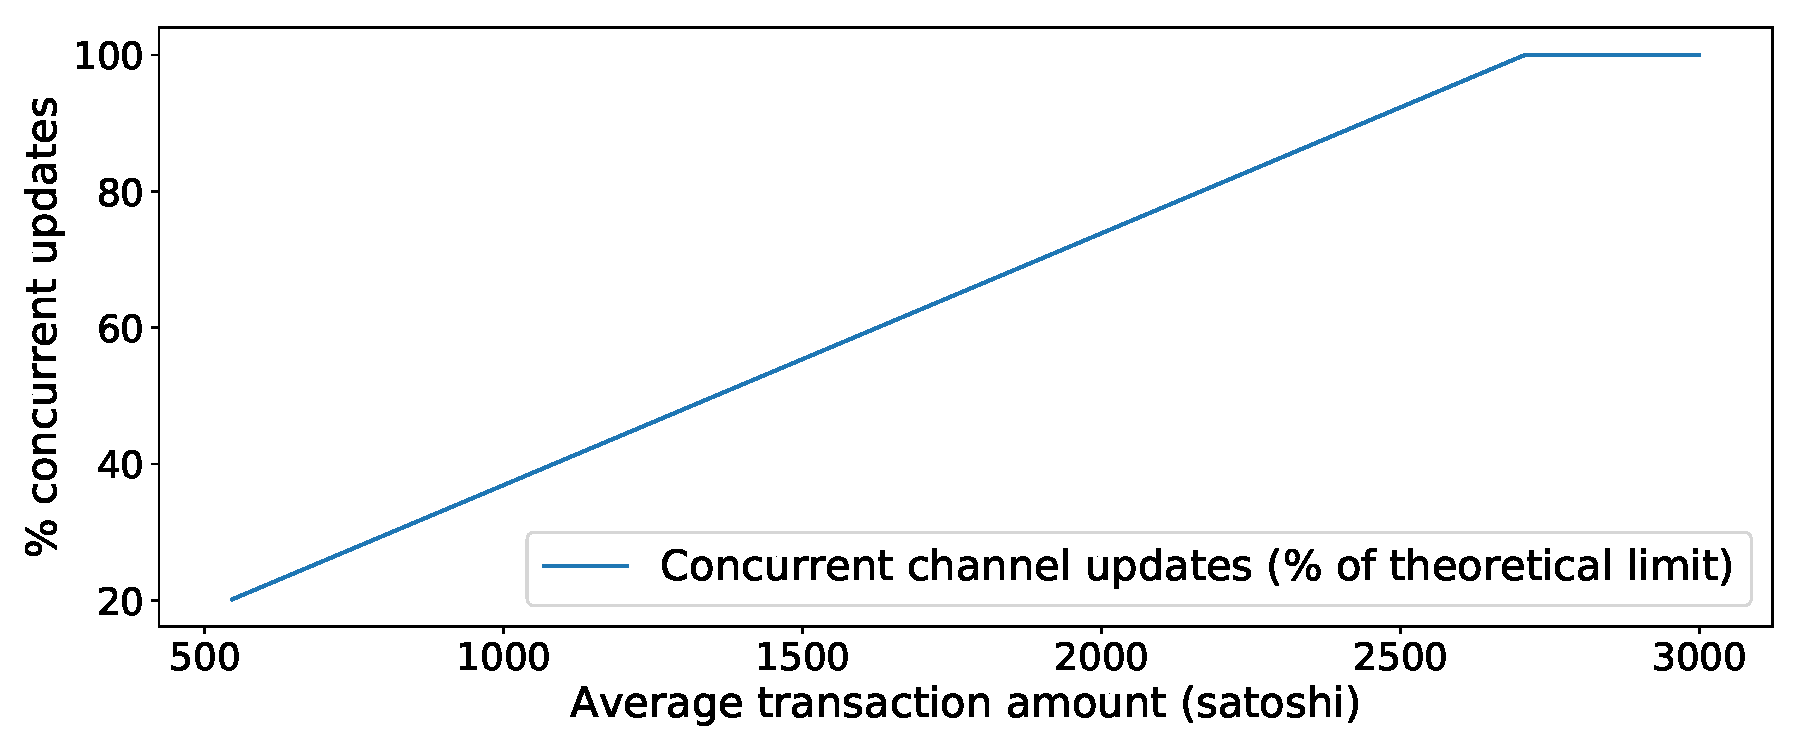
\includegraphics[width=0.8\columnwidth]{effective-channel-updates}
	\caption{Ratio between the current limit on concurrent channel updates and the theoretically possible capacity-based limit.}
	\label{fig:effective-channel-updates}
\end{figure}

\paragraph{Affected channels}
The $ur_\textit{eff}$ is an aggregated measurement that does not shed light on how the issue affects individual channels. 
Given that, we now study how many channels are affected by the HTLC limit.
The number of affected channels depends on the average transaction amount $a_\textit{avg}$.
For high values of~$a_\textit{avg}$, it is more likely that the effective update rate of a channel is limited by its capacity, whereas the HTLC limit would determine the update rate cap for small values of~$a_\textit{avg}$.
We quantify this as follows.
Given a fixed average transaction amount $a_\textit{avg}$, we consider a channel \textit{affected} by the HTLC limit if $u_{\textit{HTLC},a_\textit{avg}} < u_{\textit{cap},a_\textit{avg}}$, i.e, $u_{\textit{eff},a_\textit{avg}} < 100\%$~(\cref{fig:affected-channels}).

\begin{figure}[tb]
	\centering
	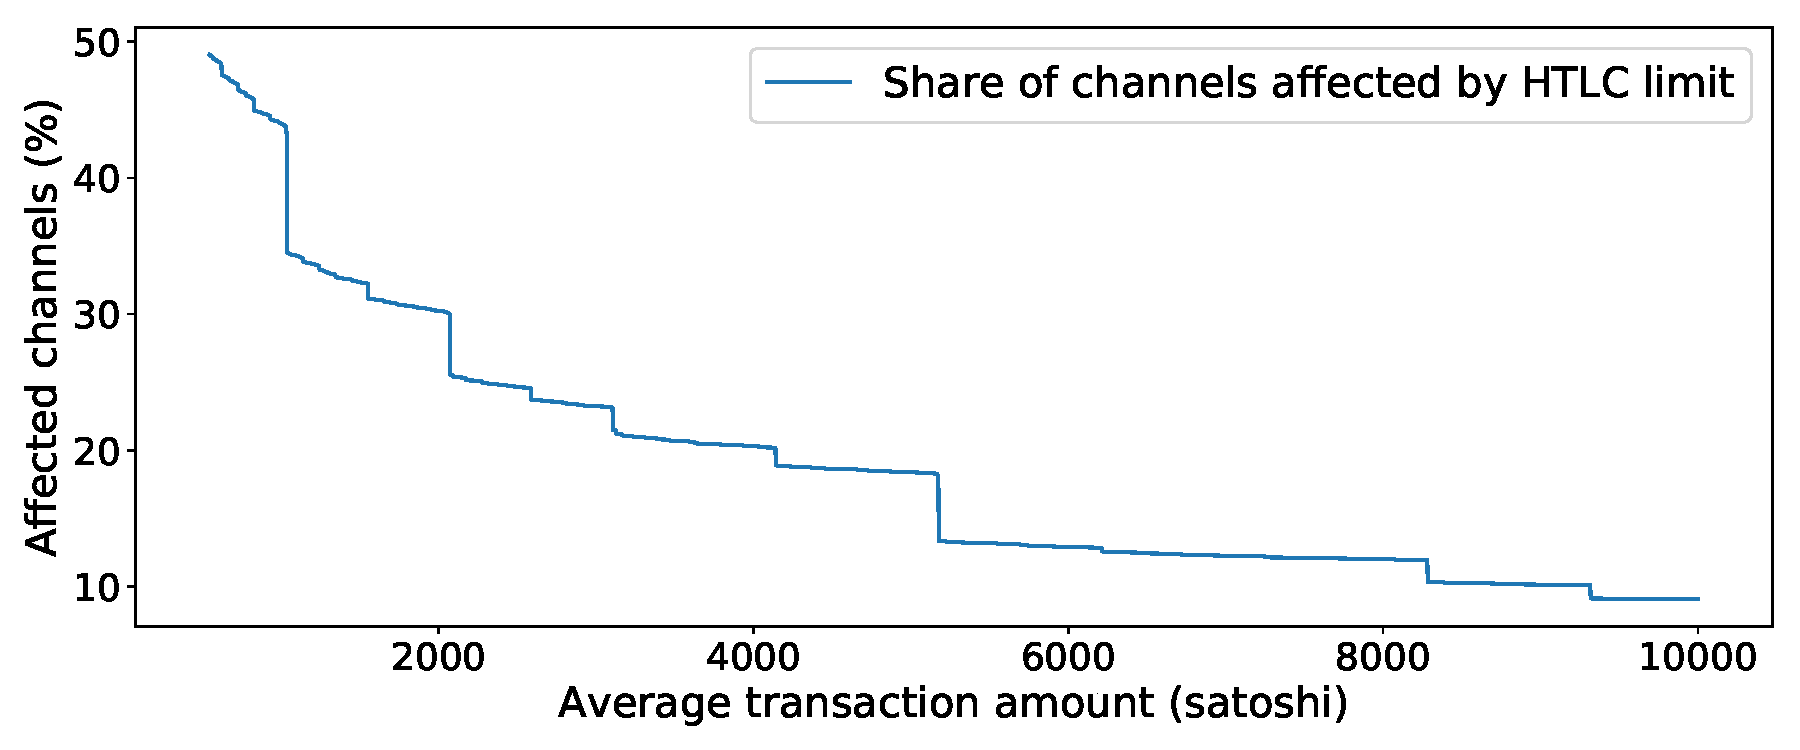
\includegraphics[width=0.8\columnwidth]{affected-channels}
	\caption{Share of affected channels for different transaction amounts.}
	\label{fig:affected-channels}
\end{figure}


\paragraph{The effect of the HTLC limit over time}

We study the effect of the HTLC limit on the LN using our historical snapshots \emph{LNHist}.
For each monthly snapshot and four assumed average transaction amounts, we calculate the share of channels affected by the HTLC limit (\cref{fig:historic-htlc-limited-share}).
As expected, the HTLC limit becomes a more pressing issue with smaller transaction amounts, if they are higher than the dust limit.
We also observe that the share of affected channels has been increasing in the early months of LN and has remained stable since mid-2019.

We finally study how the \textit{borderline amount} has changed over time.
As~\cref{fig:historic-borderline-amount} shows, the HTLC limit finds its inflexion point in transaction amount at approximately $2500$~satoshis, with the borderline amount stabilizing in mid-2019, after the initial growth.

\begin{figure}[tb]
	\centering
	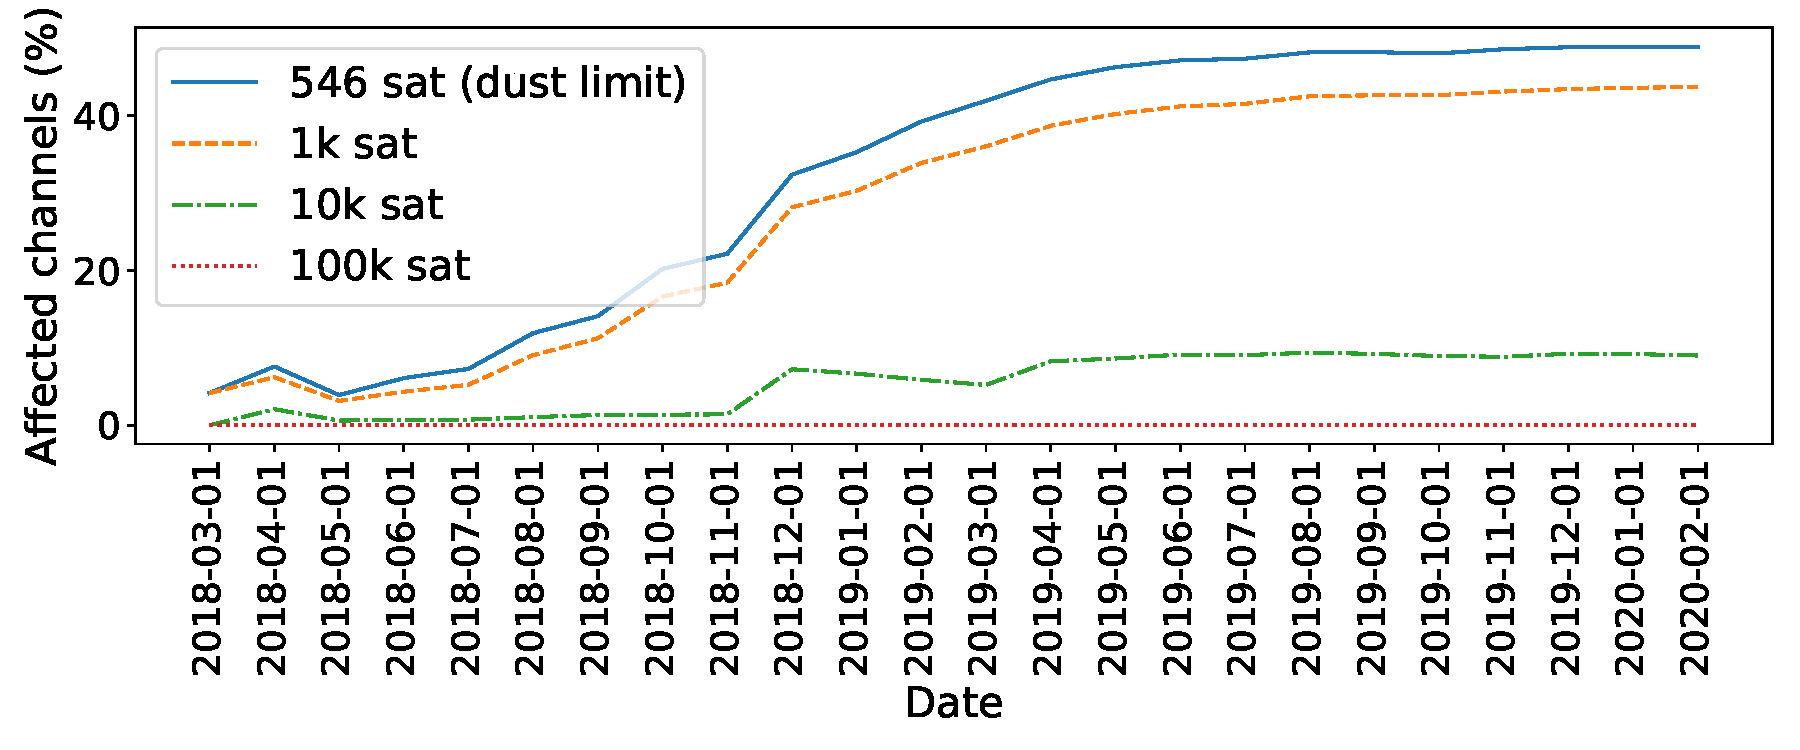
\includegraphics[width=0.8\columnwidth]{historic-htlc-limited-share}
	\caption{Historic share of HTLC-limited channels.}
	\label{fig:historic-htlc-limited-share}
\end{figure}

\begin{figure}[tb]
	\centering
	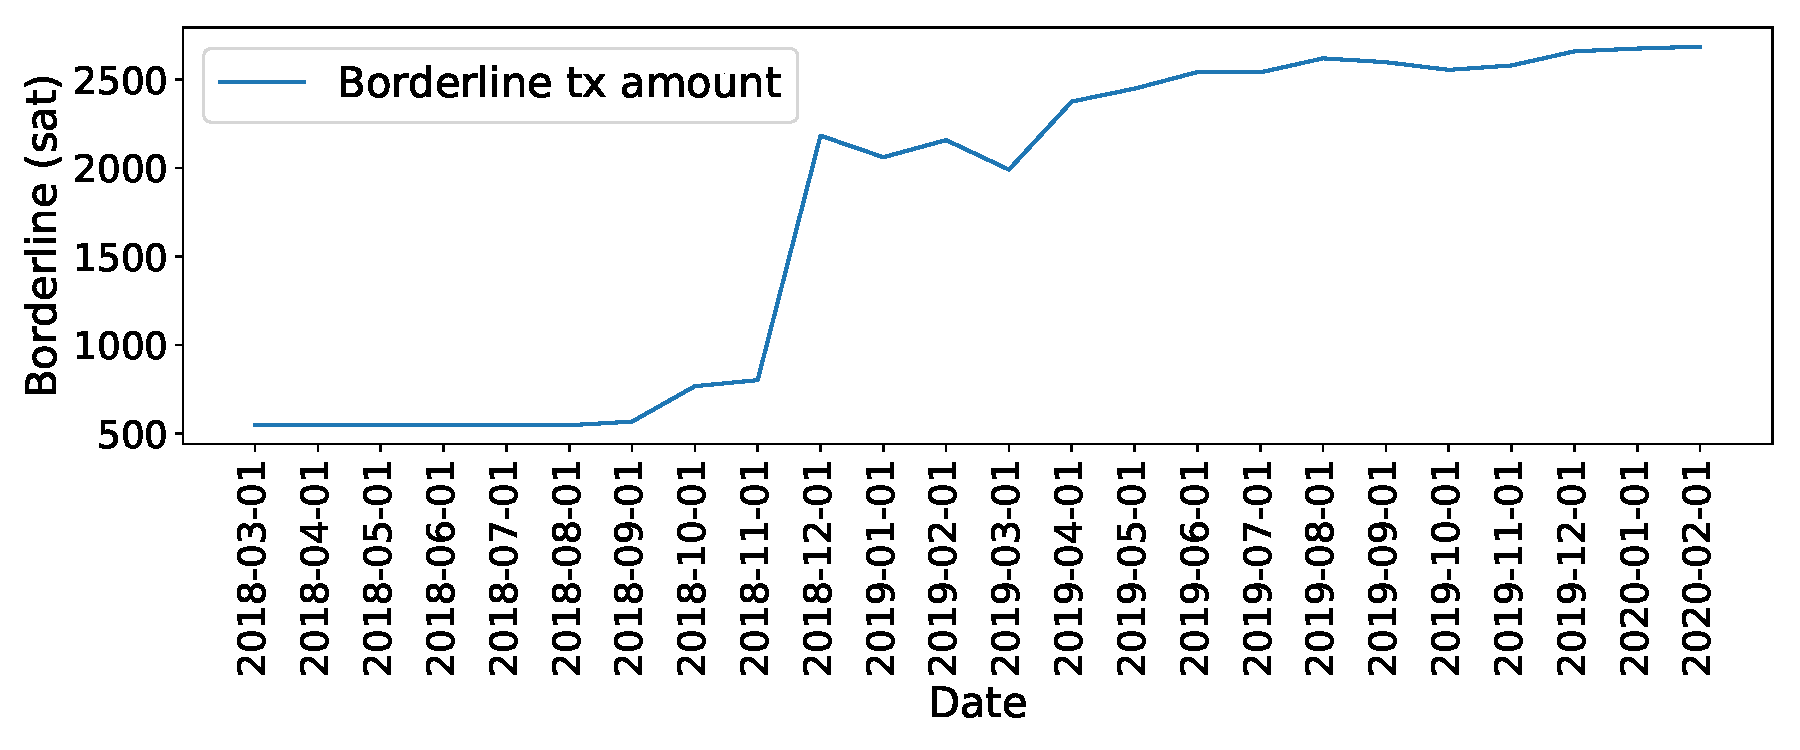
\includegraphics[width=0.8\columnwidth]{historic-borderline-amount}
	\caption{Historic borderline amounts.}
	\label{fig:historic-borderline-amount}
\end{figure}


\section{Depleting the Lightning Network}

The HTLC limit opens up the possibility of a network-wide DoS attack.
An adversary connects to both endpoints of the target channel and forwards multiple small payments to itself, but does not finalize them.
After $966$~HTLCs are added, the channel loses its ability to forward payments, until some HTLCs expire.
The attacker can thereby deplete a channel, making it unusable.

The cost for this attack depends on the minimum transaction amount.
We assume it equal to the dust limit of~$546$~satoshis (the default value in 2 out of 3 major implementations).

We calculate the total capital requirements for an attacker to block the complete LN\@.
To block all $31084$~channels, the attacker would send, in the worst case, $966$~transactions of~$546$~satoshi to each channel.
This brings the total capital requirements to approximately $163.9482$~BTC ($1.64M$~USD).

Each HTLC defines a timeout, after which the funds are returned to the sender, if the receiver provides no preimage.
From our dataset, we see that HTLC timeouts are long: $75.44$~blocks on average.
At a block creation rate of~$10$~minutes per block, this implies that an average HTLC can block the capacity for around $12$~hours.
This implies that the attacker can render channels useless for around $12$~hours using the same HTLC parameters as regular LN users.

While this rough upper bound estimate suggests a rather high attack cost, the following optimizations make it more affordable.


\paragraph{Targeting highest-capacity channels}
The attack impact can be maximized by targeting highest-capacity channels.
For example, it requires $0.05$~BTC to block 10~top channels with combined capacity of~$17.91$~BTC (\cref{fig:block-top-channels}).

\begin{figure}[tb]
	\centering
	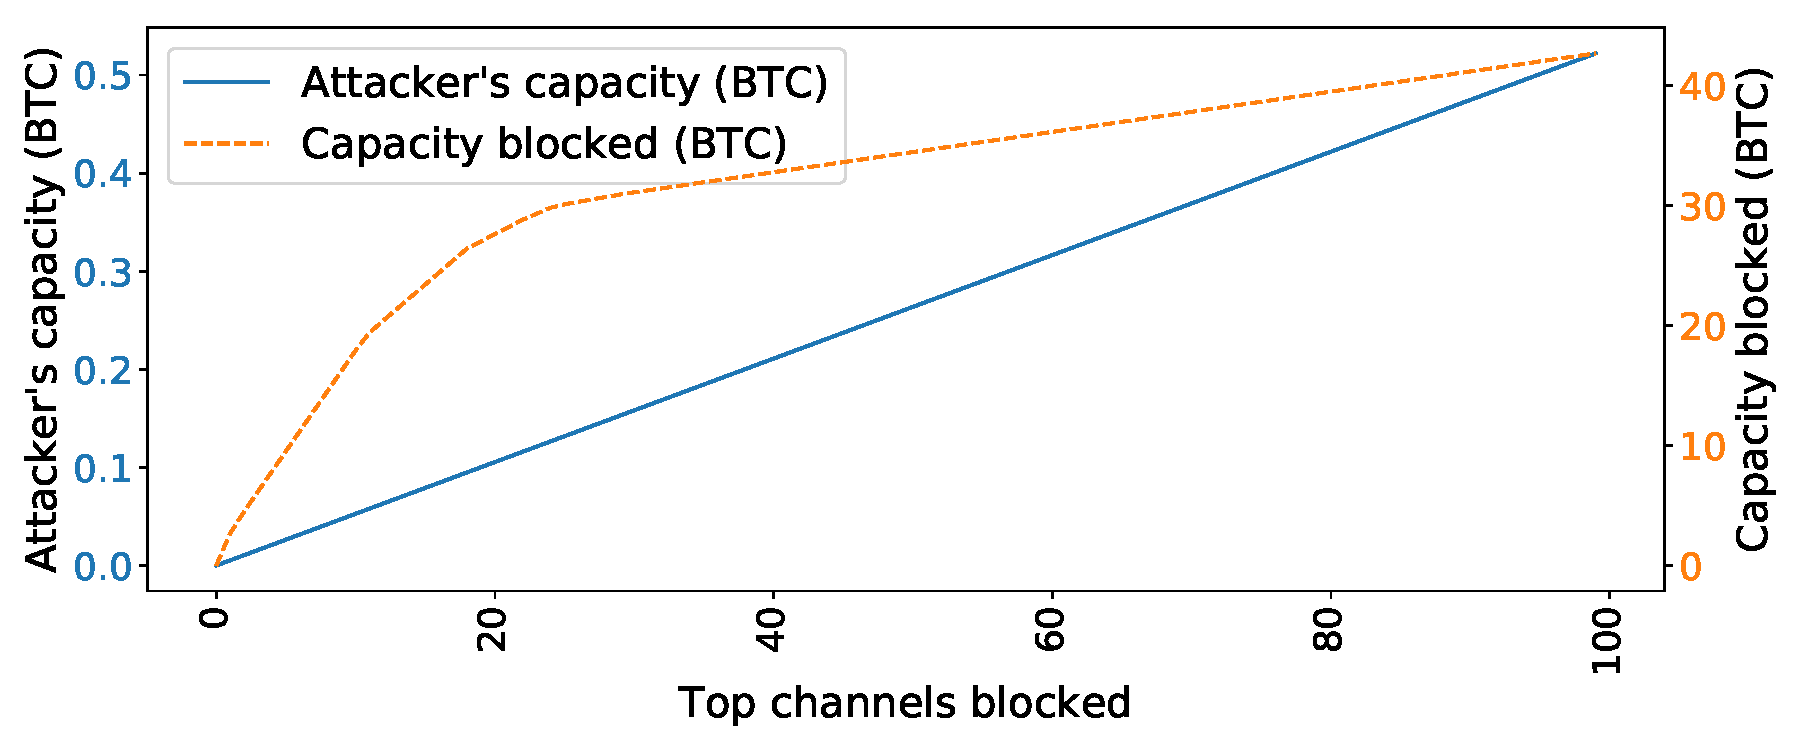
\includegraphics[width=0.8\columnwidth]{block-top-channels}
	\caption{Effectiveness of targeting highest-capacity channels.}
	\label{fig:block-top-channels}
\end{figure}

\paragraph{Real HTLC limit}
Our calculations above are based on the maximum number of concurrent HTLCs ($483$) as defined by BOLT specifications.
LN implementations may choose lower default values for this parameter.
In particular, Eclair and c-lightning enforce a lower default HTLC limit ($30$).
This means that in the real network the attacker needs to create fewer HTLCs to block channels between c-lightning and Eclair nodes as opposed to theoretical calculations and LND nodes (which by default support $483$~concurrent HTLCs per channel).
LND makes up $91\%$~of the nodes in the network, and Eclair is another $1\%$~\cite{Mizrahi2020}.
That brings real average HTLC limit to $442.23$~and lowers the attack cost by~$8.44\%$.

\paragraph{Multi-hop transactions}
The estimation above assumes single-hop transactions.
An attacker can leverage multi-hop transactions to multiply the effect of the committed capital, connecting to both ends of a $20$-hop~\cite{Bolt4OnionRouting} payment path and performing a payment to itself that never gets completed.
This is similar to capacity-based griefing attacks~\cite{HerreraJoancomarti2019}, but with much lower capital requirements.

\paragraph{Optimizing the attack based on communities}
The attacker may wish to prevent different parts of the network from transacting to each other.
To evaluate this possibility, we first divide the network into \textit{communities} using the Clauset-Newman-Moore greedy modularity maximization algorithm~\cite{Clauset2004}.
Then we consider a scenario where the attacker tries to block the channels that connect communities rather than channels within communities.
For a chosen number $N$~of the largest communities, we calculate how many channels the attacker has to block to split the network into at least $N+1$~parts: the $N$~largest communities and the rest of the network (\cref{fig:isolate-communities}).
We observe, e.g.,~that the attacker needs to block $4670$~channels ($13\%$~of all channels) to isolate the largest community from the rest of the network, locking up $25$~BTC ($225k$~USD) -- or just around $2.8\%$~of the total LN capacity.

\begin{figure}[tb]
	\centering
	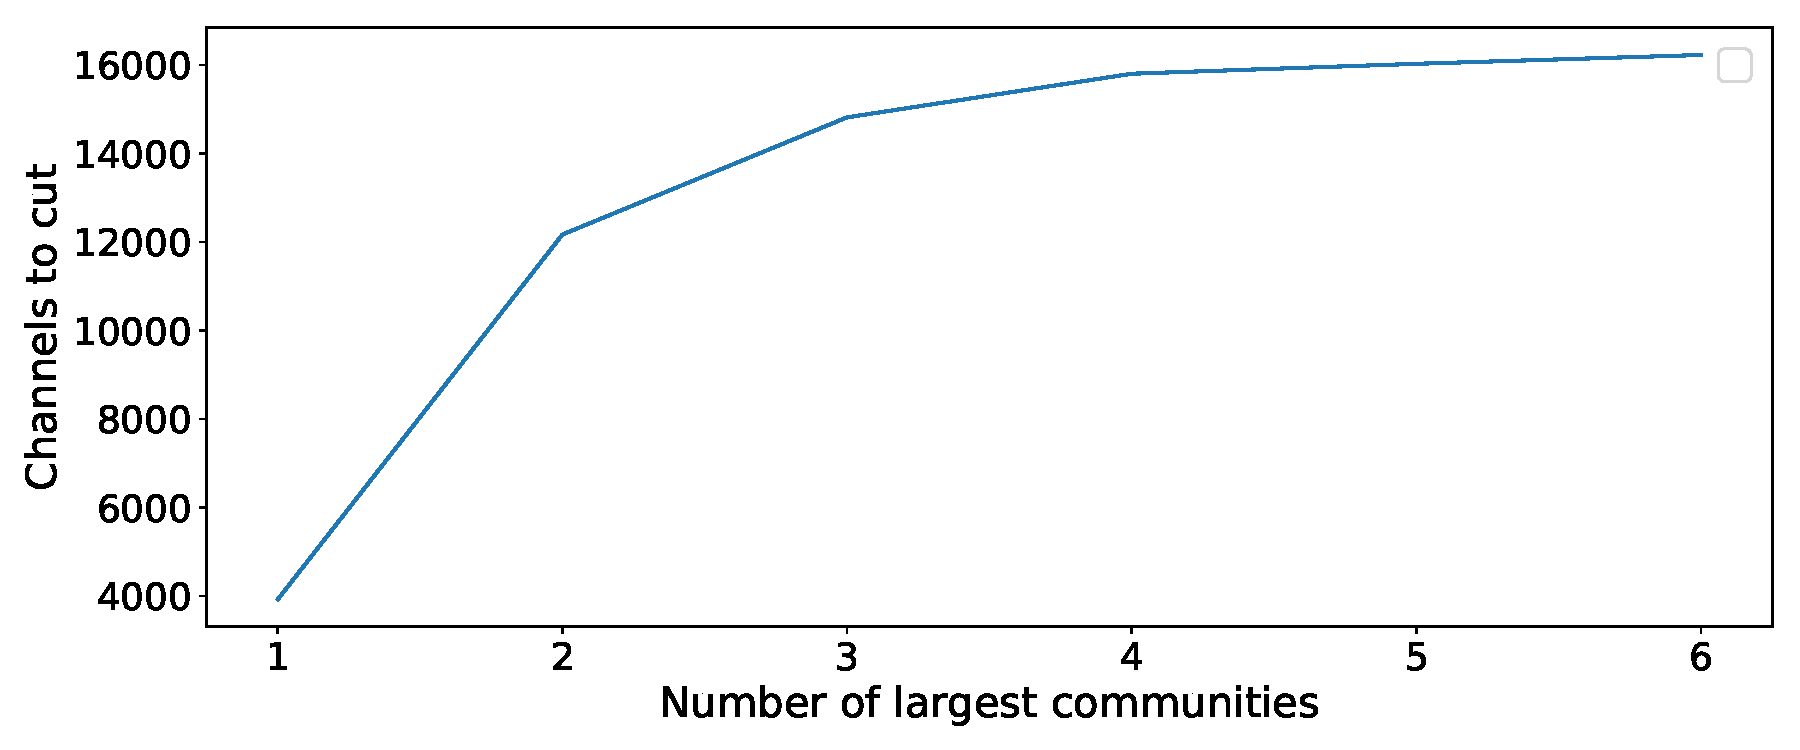
\includegraphics[width=0.8\columnwidth]{isolate-communities}
	\caption{Number of channels to cut to isolate the largest communities.}
	\label{fig:isolate-communities}
\end{figure}


\section{Discussion}
Our simplistic model does not fully reflect all the details of transaction handling.
In particular, we do not account for the fact that transactions take multiple hops (and multiple failed paths) before succeeding, nor do we reflect the unequal forwarding ability of a unit of capacity at a well-connected node, as opposed to a poorly connected one.
We also do not account for non-public channels, which may account for $28\%$~of all channels~\cite{BitMEXPrivateChannels}.
Yet, our approach allows us to calculate the effect of the HTLC limit, as both estimations (capacity-based limit and HTLC limit) are calculated under the same assumptions.
Our estimation shows that the HTLC limit reduces the number of concurrent channel updates for payments under certain average transaction amount.

The fact that the HTLC limit manifests itself at low transaction amounts negatively affects scalability and some potential LN applications, such as paying for online content~\cite{Poon2016}, which involve transactions with small amounts. 
Our calculations show that for payments of~$1000$~satoshis ($0.009$~USD), the network-wide rate of concurrent channel updates is $60\%$~lower than it could have been based solely on capacity limitations.

The low value for the default minimum transaction amount and the reduced number of in-flight transactions open a DoS attack vector with a moderate cost for the adversary.
Note that the capital in the attacker's channels will be recouped after the HTLCs time out.
Moreover, the unequal distribution of connectivity in the current LN paves the way for optimized attacks where the attacker focuses on high-capacity or inter-community channels to disrupt the seamless transfer of value across the network.


\section{Countermeasures}
One of the limiting factors for transaction throughput is the total available capacity.
This limitation is overcome by opening new channels, a countermeasure that will be naturally implemented with the growing LN adoption.
The issue of the HTLC limit is more challenging as it comes from the limitations of the Bitcoin and Lightning protocols themselves.
Therefore, more fundamental changes are needed to reduce the information required to carry out the functionality encoded in HTLCs.
One countermeasure involves replacing HTLC with AMHL~\cite{Malavolta2019}.
While HTLC requires including a digital signature, a hash value and a timelock, AMHL contract only requires the digital signature and the timelock while providing the same functionality.

This countermeasure would reduce the number of bytes required per in-flight transaction and increase the number of payments handled concurrently.
While not removing the limitation on the number of concurrent transactions, this countermeasure raises this limit, reducing its negative effect on LN scalability.


\section{Conclusion}

We quantitatively analyze the negative effect on scalability produced by the limit on concurrent payments in the LN\@.
We calculate that the limited concurrency in the LN implies that an adversary can block the complete LN investing around $1.5M$~USD ($18.5\%$~of the network capacity).
In comparison to~\cite{PerezSola2019}, our HTLC depletion attack achieves the same result (a victim node can not forward payments), but exploits the HTLC limit at each channel rather than its capacity.
Compared to~\cite{Mizrahi2020}, we properly account for the way LN handles payments below the dust limit.
The attack cost can be substantially reduced by targeting highly valuable channels (e.g., high-capacity channels or those connecting the biggest communities in the network).